% background chapter continued
\section{Mercator Architecture}\label{blueprint}
This section proceeds into detailed description of Mercator\cite{mercator} web crawler surveyed in section \ref{relatedworks}. Figure \ref{fig:basicarch} is a high-level composition of the same. As seen, Mercator specializes different steps defined in basic crawling
algorithm covered in section \ref{basicalgo} and adds several other steps to address
the social and scalability challenges of web crawler. Its blueprint design offers
horizontal scalability and therefore if implemented can run on more than one node.
Each part that contributes to mercator crawler can also be referred to as a
component, module, subsystem, etc. They can be used interchangeably from this point onward.

\begin{figure}[h!]
  \centering
  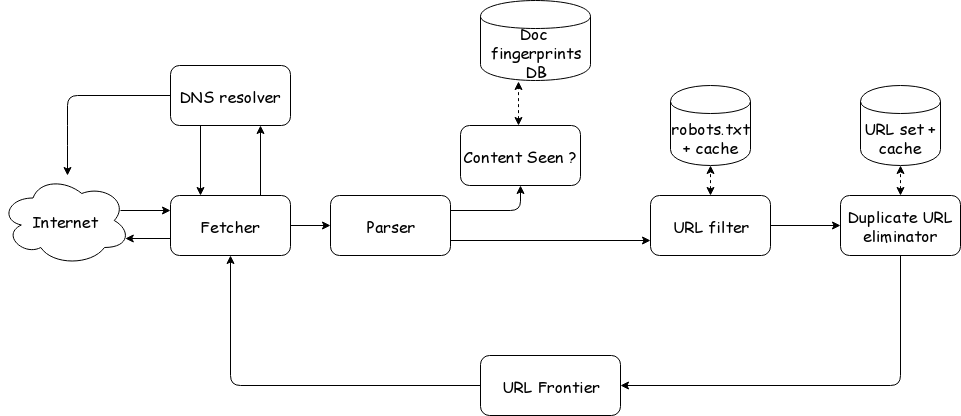
\includegraphics[width=16cm,height=14cm,keepaspectratio]{../media/crawler/basic-crawler-architecture-v2.png}
  \caption{High-level organization of Mercator}
  \label{fig:basicarch}
\end{figure}

\noindent
Each work cycle begins and ends at the URL Frontier. Depending on what needs to be
achieved, the entire crawler can run as a single process or can be partitioned into multiple processes - treating each subsystem as a process. Given a single URL, it
goes through the cycle of being fetched followed by passing through various checks,
filters and eliminations, then finally returned to the Frontier (for incremental crawling).
\\
\\
At the beginning of each logical loop cycle, a worker thread pops a URL from the Frontier data structure adhering to the priority and politeness policy. The output URL is then fetched by HTTP fetcher subsystem - which like any other web client contacts DNS module to get IP address of the corresponding web server. The web page is then retrieved and stored at a temporary location which is then picked up by parser subsystem which forwards the path to the page and extracted links to content seen and URL filter, respectively. The batch of URLs undergo a fixed set of pre-processing steps at the URL filter subsystem before being passed over to Duplicate URL eliminator (DUE). The DUE module tests each URL to determine whether the link should be added to the
URL frontier.

\pagebreak

\subsection{Fetcher, Parser, and DNS}\index{Fetcher, Parser, and DNS}
It occurred to designers of Mercator that the task of fetching each URL from seed set or newly discovered
links is complex. First, the request made to the web server at a given URL endpoint will have several outcomes as a response. Therefore, it becomes a bottleneck to implemented fetcher as only single threaded, blocking synchronous module. Instead it should be written as a multi-threaded, synchronous I/O or non-block,
asychronous I/O to speedup the operation. Moreover, it is also inefficient to have DNS resolve a given URL's
IP address each time a fetch request is made to the same web server. This can be fixed by having a cache of
lookup pair for each web host in the frontier. According to Mercator designers, another difficulty is the lookup implementation itself of DNS entries is blocking; meaning that at a time only one request is considered and completed and all other requests queue up. The solution for this is yet again a multi-threaded approach
or a asynchronous I/O wrapper.

\subsection{Handling De-duplication}
Any professional or sophisticated crawler has the capability to minimize De-duplication. De-duplication
simply tests whether a web page with the same content has already been seen at another URL. As per
figure \ref{fig:basicarch}, the content seen subsystem takes care of the same. There exist three
established methods to solve this problem. 

\begin{description}
\item[Document Fingerprinting(checksums)] \hfill \\
  A digital fingerprint uniquely identifies a file by mapping large data inside a file to a shorter
  string. This method is straight forward way to control data duplication. Widely deployed fingerprinting
  functions are one-way cryptographic hash functions such as \textit{MD5}, \textit{SHA}, and
  \textit{bcrypt}.However, this simplistic approach fails to detect near duplicates which is much needed
  for tools like crawlers\\ 
\item[Bloom Filter] \hfill \\
  This is a data structure which gives a probability of same document being already present in the data
  store. One downside is sometimes it also gives false positives, meaning, the filter outputs saying
  `the document already exist but in fact it doesn't`. This can be used for avoiding near duplicates but
  at the cost of missing unseen files due to false positives. This can be tackled by some application
  strategy.
\item[Shingling] \hfill \\
  In many cases, the contents of one web page is similar to other differing only by few keywords, for
  example - the published date and time. This technique does textual analytics to detect near duplicates.
  Shingles\cite{dedupe} improve over \underline{bag of words} technique because it ignores the context of
  words. Shingling overlaps phrases of neighboring few words at a time much like shingles on a roof.
  \underline{Minhash} and \underline{Simhashing} are best known non-trival implementations for
  near-duplicate detection.
\end{description}

\pagebreak

\subsection{URL Filtering}\label{urlfilter}
The URL Filter component takes input a batch of extracted URLs, applies a series of tests, modifiers on each URL, composes a newer batch of URL which fall in its
criteria and forwards it to the next subsystem. For instance, assume a set of links $\{U_1,U_2,U_3,U_4,...,U_i\}$ extracted from page $p$, there is a possibility that some $U$'s link are relative to the page $p$, in
such cases, this component normalizes such $U$'s turning them into absolute URLs. Also, the crawler can
enforce a rule to exclude out of bound URls - those that don't fall within a given list of domains. 

\begin{figure}[h!]
  \centering
  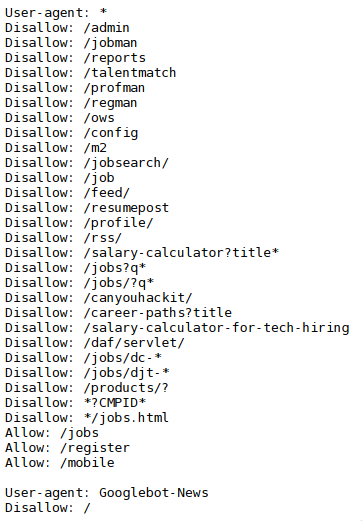
\includegraphics[width=8cm,height=13cm,keepaspectratio]{../media/crawler/robots-txt-sample.png}
  \caption{Robots Exclusion Policy set by dice.com}
  \label{fig:robotsdice}
\end{figure}

\noindent
Apart from these, many hosts regulate whats allowed/not-allowed for downloading by placing a \textit{robots.txt} file under root directory of a hosted web site. The standard is known as Robot Exclusion Protocol.
Figure \ref{fig:robotsdice} shows a \textit{robots.txt} of dice.com. Its interpretation beginning at line one goes like no crawler should visit \textit{/admin}, \textit{/jobman} pages, but it can visit \textit{/jobs},
\textit{/register}, and so on. A user-agent containing string Googlebot-news is not legally allowed to
crawl  any of its pages. For each domain, the crawler fetches robots.txt to test whether the URL under consideration passes the robot restrictions and only then it is added to its Frontier data structure. Given a
high locality that many of the extracted links fall within the domain, it is efficient to cache robots.txt rule into an in-memory data store. The cache expires and redownloads robots.txt for each domain several times a day to stay in sync with the rule changes.
\\
\\
It should be noted that it is always safer and courteous to include a note in request header of the crawler indicating intentions to download the data, and also provide your email address where the webmaster can contact you in case of any issues. Also, it is a good practice to enforce strict compliance with domain's robots.txt rules.

\subsection{Duplicate URL Eliminator (DUE)}\index{Duplicate URL Eliminator(DUE)}
A batch of URLs qualified from URL filtering subsystem arrives at DUE. Sometimes it s also referred to URL-seen test. DUE guards the URL Frontier by eliminating
multiple instances of the same URL from adding to the Frontier. It also keeps history of set of URLs that were previously added to the URL Frontier and those that are
currently in it. The fire-and-forget, one-time crawl URLs are only crawled once. In
continuous crawling Frontier scheme, some URLs are revisited periodically for new information, in such cases, the DUE has to delete its traces from its state.
\\
\\
\noindent
Understanding the behavior of DUE explained in above paragraph, the size of URL set stored in relational database on disk will grow linearly as the size of web corpus grows irrespective of whether the crawler is continuous/non-continuous. Since the DUE has to make sure that it isn't adding duplicate URL to the Frontier, it will check against each entry in the URL set table. This will hamper DUE throughput and increase disk seek latency over time i.e the time taken to check and respond for existing entry increases. Each insertion in the URL set table is a fixed size checksum of
textual URL along with the mapping to URL itself. The checksum algorithm should be
such that it has exponentially small probabilistic bounds on the likelihood of
collision in the URL set.
\\
\\
To reduce the number of operations required to DUE each URL in a batch, several
optimizations can be combined. First, keeping an in-memory cache objects of popular URLs. The intuition for this is continuous crawling URLs endpoint will be revisited. But again with this, the cache hit rate is low as ratio of continuous to one-time crawls can be 20:1. Also as the computed checksums of the URLs are highly unique, it has lower locality, so the checksums that miss the cache will require disk access and disk seek. Secondly, taking advantage of high locality of checksum hostname(domain name) concatenating with checksum of absolute URL for that domain name results in
same host names being numerically closer to each other. This in turn translates to
access locality on the URL set.

\pagebreak

\subsection{URL Frontier}\label{scheme}
The URL Frontier subsystem receives a batch of URLs from its counterpart(it is either DUE or hostsplitter in case of Distributed crawling). It maintains those URLs in the Frontier and propagates them in some order whenever the fetch module seeks a URL from it.

\begin{figure}[h!]
  \centering
  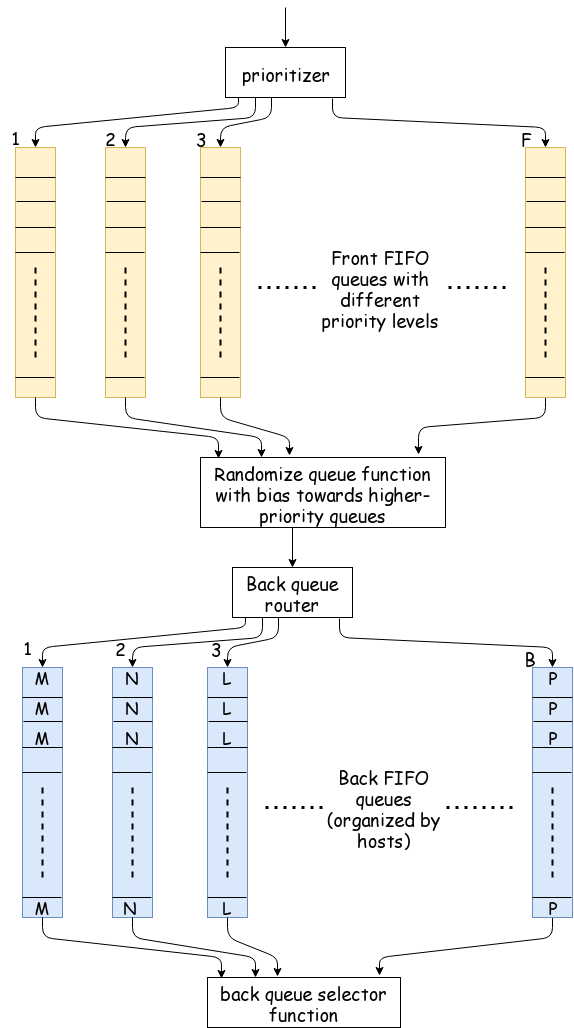
\includegraphics[width=12cm,height=15cm,keepaspectratio]{../media/crawler/url-frontier.png}
  \caption{URL Frontier Scheme(based on Mercator)}
  \label{fig:frontier}
\end{figure}

\noindent
Figure \ref{fig:frontier} is not just a simple queue but a complicated data structure. It includes multiple pages from the same host. It avoids trying to fetch all those pages from the same host at the same time because may be the crawler can overload the server which is not a good policy. Also, the fetch module should not wait doing nothing, instead keep the module busy. Thus, it balances the tradeoff between not
bombarding the server and also keeping the fetch module busy so that if fetch is not crawling that website
at least it can go to some other server and fetch some pages from there.

\pagebreak

\noindent
Following are important considerations that dictate the order in which the URLs are returned or pulled from
the frontier. As mentioned earlier, simple priority queue fails as there is high locality of pages that go
to its own site, creating a burst of accesses to that site.

\begin{itemize}
\item \textbf{Explicit politeness:} obeys any specifications from webmaster on what portions of the site
  site can be crawled, see section \ref{urlfilter} for more details.
\item \textbf{Implicit politeness:} Avoids hitting any site too often even though no specification exist
  on the site.
  \item \textbf{Freshness:} crawl some pages more often that others.
\end{itemize}

\noindent
A common heuristic to handle politeness is to insert a time $t$ gap between successive requests $r$ such
that,
\begin{align*}
  t(r_i) &> t(r_{i-1}) \\
  t(r_i) &= (K.l(r_{i-1})) + TS && \text{...$K$ is a variable delay factor}
\end{align*}

\noindent
meaning the time taken by successive request $t(r_i)$ is order of magnitude larger than time taken by
most recently fetched $t(r_{i-1}$ request. $K$ is the Crawl-Delay attribute found in web hosts robot-exclusion protocol. It varies
from host to host and its presence is basically to inform target crawler agent that it may revisit the
host in integer N, where N is usually seconds. On web servers where this attribute is not specified,
general rule of thumb is to set K to 10 sec. $l(r_{i-1})$ is the latency of the request and $TS$ is the
timestamp. $K$, $l$, and $TS$ is the time buffer which is specific to this thesis crawler implementation
and is the earliest time $t(r_i)$ at which the host can be hit again.
\\
\\
\noindent
It is important to visualize URL Frontier diagram figure \ref{fig:frontier} before diving into its pieces. A URL follows the path into the Frontier and immediately encounters set of front queues $F$. It enters into one of these $F$ queues. There are also another set of queues called $B$ back queues. At some stage the URL will be pulled out of the front queue and then sent into one these back queues. Later, at some stage, it will be pulled out of that back queue and accessed by fetcher thread which then goes and actually fetches
the document at that URL endpoint.
\\
\\
\noindent
Each front queue $F_m$ in range $\{1,2,3...m\}$  and back queue $B_n$ in range $\{1,2,3,...n\}$ is literally a $FIFO$ queue. The incoming URL gets classified into one of the ${1,2,3,..F}$ front queues

\begin{itemize}
\item \textbf{Front queues} $F_m$ manage prioritization. They influence the rate at which you ping the
  same web server again and again.
  \item \textbf{Back queues} $B_n$ enforces politeness.
\end{itemize}

\pagebreak

\begin{figure}[h!]
  \centering
  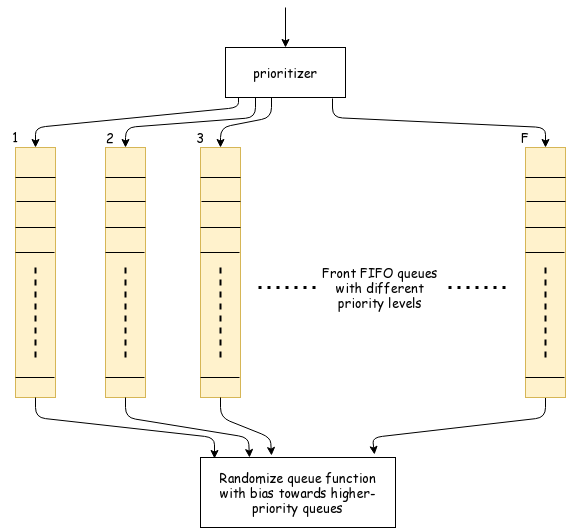
\includegraphics[width=14cm,height=12cm,keepaspectratio]{../media/crawler/f-queue.png}
  \caption{Frontier Front Queue}
  \label{fig:fqueue}
\end{figure}

\noindent
Figure \ref{fig:fqueue} gives a close inspection on Front Queues $F_m$. Incoming URL is assigned a integer  priority between 1 \& $m$. Based on the priority assigned it is going to enter that particular queue.
priority $F_1$ holds URLs for web servers that need to be crawled very very frequently. For instance,
let $L_s$ be links, $\forall L_s \in $ \textit{dice.com} $ \longmapsto $ $F_1$ has highest crawling requirement whereas $\forall L_s \in $ \textit{jobs.com} $ \longmapsto $ $F_m$ contains URLs which has least
crawling requirement. 
\\
\\
Heuristics for assigning priority,
\begin{itemize}
\item keeping track of how frequently the web pages are changing on a particular web server and how authoritative the pages are, if it occurs a case where a refresh rate is pretty high for any web server and pages happen to be important enough then those web servers are going to be crawled more often
\item Application specific. 
\end{itemize}

\noindent
The prioritizer function for whirlpool is explained in chapter \ref{implwhirlpool}, subsection \ref{priotizer}.Also randomize queue strategy on how the items get pulled out of this $F$ Front queues is explained in chapter \ref{implwhirlpool}, subsection \ref{fqbiased}. This sums the top half of the picture.

\pagebreak

\noindent
The back queue $B$ exist to achieve politeness because the crawler shouldn't hit the server too frequently.
Again, there are $B$ back queues from $\{1,2,3,...n\}$, so when the URLs are pulled out in biased order from $F$ Front queues, they are going to enter into one or more of these back queues. 

\begin{figure}[h!]
  \centering
  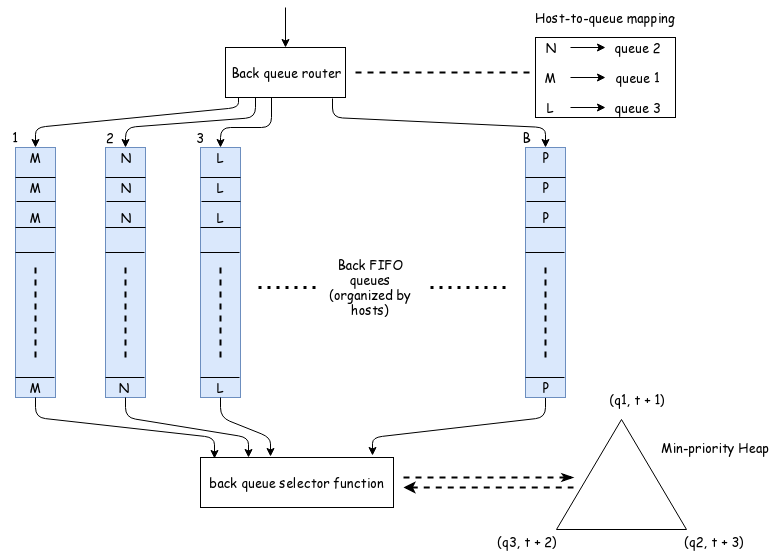
\includegraphics[width=15cm,height=13cm,keepaspectratio]{../media/crawler/b-queue.png}
  \caption{Frontier Back Queue}
  \label{fig:bqueue}
\end{figure}

\noindent
Recall the heuristic to handle politeness explained earlier, each back queue $B_n$ corresponds to a particular domain. For e.g back queue $B_1$ is for server \textit{monster.com}, $B_2$ could be the server \textit{indeed.com}, and so on. So all the URLs which have base name \textit{dice.com}, when they emerge from the front
queue enter queue $B_1$. Furthermore, Back queues maintains a minimum priority heap data structure in which
the keys are such that the parent key $k$ is less than the key of both of its children i.e $k < 2k$ and $2k+1$ and so the smallest item in the heap is at the root of the heap.
\\
\\
The size and vertex $V(q,t)$ of the heap is B. the key $q$ from vertex pair $(q, t)$ in it maps to one of the servers/back queues $B_n$. The value $t$ is going to be threshold timestamp $th_{ts}$ which is the value
of time before which I am not allowed to hit the same server $B_n$ again. The very fact that back queue structure maintains a minimum heap is that its particular root represents the server which has the least value
of the timestamp. Its the very server that is allowed to query next before it queries any of those other servers. A URL $u$ is pulled out from the head of server queue $q$ and fetched by fetch module. This is handled by back queue selector function
\\
\\
While this cycle continues, the back queue router ensures the server queues $B_n$ are non-empty.  It is busy with pulling a URL $u`$ from the head of front queue picked up by some randomize front queue function. Following this, it checks whether server queue $q$ exists for $u`$, if so, then it gets added to that queue. It goes again to pull another URL $w$, this time it sees that server queue $q$ is now empty and there insert $w$ in it and renames the $q$ to $q`$. During the same iteration, the process sinks a new vertex
$V`(q`,t`)$ on to the min-heap based on the meta-information of $w$ such as time $t`$.



\pagebreak

\subsection{Distributing Web Crawl}\index{Distributing Web Crawl}
A crawler program as a whole can be distributed for various reasons. A distributed crawler can crank up crawling rate. This is achieved by making a identical clone of single node crawler and replicating it onto another machine. Another advantage of distributing the crawl is that a subset of websites are crawled by a machine which is geographically closer to its data center/region. The immediate question is how does mercator extend its architecture and also how do these nodes communicated and share URLs is shown in figure \ref{fig:hpart}.

\begin{figure}[h!]
  \centering
  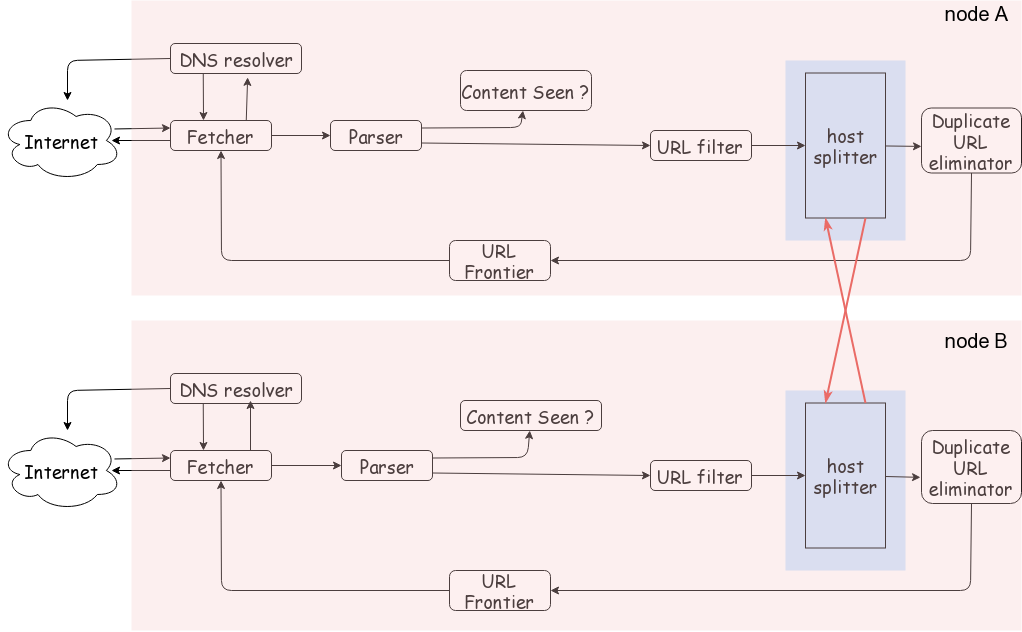
\includegraphics[width=15cm,height=9cm,keepaspectratio]{../media/crawler/host-splitterv3.png}
  \caption{Host Partitioning}
  \label{fig:hpart}
\end{figure}

\noindent
Lets say there are 3 different nodes designated to crawl the web $M_1, M_2, M_3$. All
the hosts that are being crawled are partitioned into 3 sets. Imagine taking every
single web server on the web or in the seed set, taking the URls for those servers, and hashing those URLs in the integer range $i \in \{1,2,3\}$. For instance, web
server address \textit{usjobs.com} could get hashed to an integer 2. So all those URLs that are being stored by that web server will be parsed by node $M_2$ while the other two nodes do not fetch documents located on \textit{usjobs.com}.
\\
\\
The key to the implementation is the host splitting component shown in figure \ref{fig:hpart}. The component at machine $M_1$ computes which machine is meant to crawl
the URLs of \textit{usjobs.com}. It takes the URL, looks at its server's address and
hash it to the integer 2 upon which it knows $M_2$ is supposed to crawl URLs located
on this server and therefore sends it to node $M_2$. Looking at the snapshot of node $M_2$, it has passed content seen, URL filter tests which confirms the incoming URL
from different node is valid and need not go through the tests again. The only thing node $M_2$ has to check is whether that URL already exists in its own local URL frontier version or its own DUE. If the URL is new, the node will add it to its own URL
frontier. At the same time node $M_1$ simultaneously receives URLs that it is supposed to crawl from those other nodes $\{M_2, M_3\}$.

\pagebreak